\section{The Spring Framework}\label{sec:spring-framework}
The Spring Framework is used for the backend of the implementation. Information on the
framework was mostly taken from~\citep{springframework, johnson2004spring}, as well as~\citep{walls2022spring}. They can be looked at for
further reference. Code examples are taken from our project.

Spring is an open-source framework for building Java applications. It also supports the Kotlin programming language, which has been used for our
implementation. The first release was in 2002 and the latest version, at the time of writing, is Spring Framework 6.0. It is extremely
lightweight (both in size and overhead), being distributed in a file of just over 1 MB\@.

The framework is split into many modules that are grouped into several layers. We do not have to use each one of the modules but choose them
according to the application's architecture and requirements. All modules are built on the top of the core container which includes the
configuration model and a dependency injection mechanism.

\Cref{fig:figure4.6} shows all the Spring layers and modules, and what each of them does is briefly explained below.

The Spring Framework module layers include:

\begin{enumerate}
    \item Core Container -- includes four modules, with Beans and Core providing the integral functionality of the framework -
            IoC (\emph{Inversion of Control}) and DI (\emph{Dependency Injection}).
    \item Data Access/Integration -- includes five modules used for data handling and integration. One of them is ORM (\emph{Object Relational
            Mapping}) which provides several object-relational mapping APIs, including JPA (\emph{Java Persistence API}), which we use in our
            implementation.
    \item Web -- this layer includes four modules. One of them, Web, is used in our implementation and it provides web-oriented integration
            features.
    \item AOP, Aspects, and Instrumentation -- AOP module provides aspect-oriented programming implementation, while the Aspects module
            supports integration with AspectJ. The instrumentation module provides class instrumentation support which is used in some
            application servers.
    \item Test -- this module, as the name states, supports testing of the components with JUnit or TestNG\@.
\end{enumerate}

\begin{figure}[hbt!]
    \begin{center}
        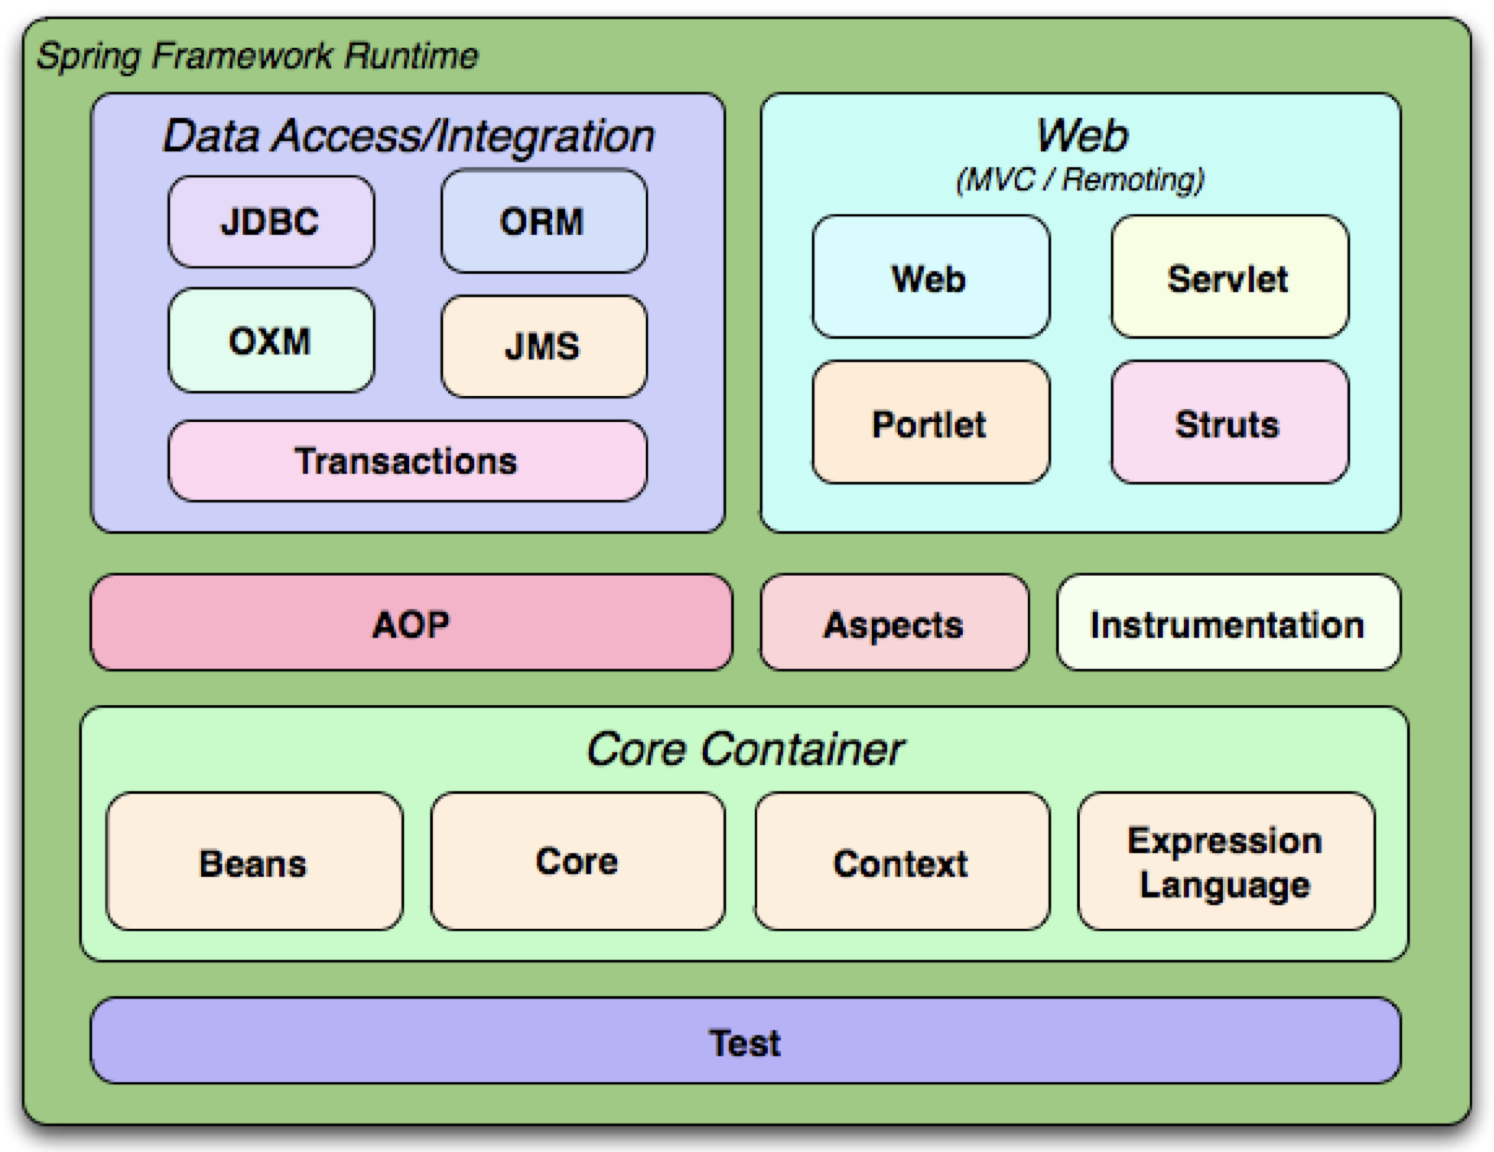
\includegraphics[width=0.9\textwidth]{graphics/4-background/1}
    \end{center}
    \caption{Spring Framework Layers and Modules~\citep{introtospringframework}}
    \label{fig:figure4.6}
\end{figure}

Since we mentioned that we use some of the modules in our implementation, namely ORM and Web, we will now explain them more in detail, as well
as the concept of dependency injection and inversion of control.

\subsection{Dependency Injection}\label{subsec:dependency-injection}

We spoke about inversion of control and dependency injection mechanisms, but what do they actually do? Inversion of control is at the core of
Spring Framework. Almost every application nowadays consists of many classes and they need to collaborate with each other. In
general, every object has to obtain its own reference to the object it is working with (its dependencies), which is not really efficient.
This is why, by applying inversion of control, objects are given their dependencies at the time they are created by an external entity. This
means that dependencies are \emph{injected} into objects. By using IoC, we invert the responsibility of how the object obtains references to
the objects it is collaborating with.

Now, an example of how to declare a CityController class in Spring whose constructor contains two private parameters will be shown.

\begin{figure}[hbt!]
    \begin{center}
        \begin{lstlisting}[language=Kotlin,label={lst:spring-code-1},belowskip=-1 \baselineskip]
@RestController
class CityController(
        private val cityRepository: CityRepository,
        private val cityMapService: CityMapService,
)
        \end{lstlisting}
    \end{center}
    \caption{Declaring a class in Spring Framework}
    \label{fig:figure4.7}
\end{figure}

When a class is declared, the constructor is simply given all the objects needed in that class. Spring gives those objects during the
creation of an instance of a class, or even the implementation if it is an interface. These objects are called \emph{beans}. A bean can take
other beans in the constructor, or can itself be given to those who require it. Beans are declared with the help of annotations such as
\texttt{@Component}, \texttt{@Service}, \texttt{@Repository}, \texttt{@RestController}, etc.

\subsection{Object Relational Mapping (ORM)}\label{subsec:object-relational-mapping}

With the use of ORM, the main goal is to avoid writing SQL statements manually. In order to do this, first an entity is defined using the
\texttt{@Entity} annotation. Below is our example of a \texttt{City} entity. This entity represents a single table row in the
database. It contains all the columns that are found in that row, such as \texttt{id}, \texttt{name}, \texttt{x}, and \texttt{y}.

The first column (\texttt{id}) is annotated with \texttt{@Id} and it represents the primary key. Using \texttt{@GeneratedValue} annotation, Spring
generates the primary key value by itself and increments it automatically in our case. The rest of the columns in this entity are annotated
with \texttt{@Column}. There are other annotations for the columns like \texttt{@OneToMany}, \texttt{@ManyToOne},\texttt{@ManyToMany}, etc.
Based on this entity, Spring will automatically generate the corresponding table.

This is an advantage of Spring since the manually written SQL was not used to create the table, thus if the database needs some changes later,
the same code will work with MySQL, Postgres, H2, and others.

\begin{figure}[hbt!]
    \begin{center}
        \begin{lstlisting}[language=Kotlin,label={lst:spring-code-2},belowskip=-1 \baselineskip]
@Entity
data class City(
        @Id
        @GeneratedValue(strategy = GenerationType.IDENTITY)
        val id: Long? = null,
        @Column
        val name: String,
        @Column
        val x: Double,
        @Column
        val y: Double,
)
        \end{lstlisting}
    \end{center}
    \caption{Example of a Spring Framework entity}
    \label{fig:figure4.8}
\end{figure}

The data in the database is accessed over the repositories. These repositories are just interfaces, not classes that need to be implemented, and
Spring creates the instance of an interface by itself. Interfaces in our project implement \texttt{JpaRepository} which already has some predefined
methods such as \texttt{findAll()} for returning all instances of the type, \texttt{deleteById()} for deleting entity with the given ID,
\texttt{save()} for saving a given entity, etc. If more complex queries are needed, the methods can be added to the interface and Spring will
automatically create the query based on the method name, its parameter types, and the return type.\footnote{More on supported query method
predicate keywords, modifiers and return types at \\ \url{https://docs.spring.io/spring-data/jpa/docs/current/reference/html/}} Examples of these
methods can be seen in the code below: \texttt{findByName()} takes the city name and returns the whole \texttt{City} object if
there is one by that name, and \texttt{deleteByName()} method. If something beyond the queries that Spring can generate on its own is needed, the
regular full SQL query can be written as well.

\begin{figure}[hbt!]
    \begin{center}
        \begin{lstlisting}[language=Kotlin,label={lst:spring-code-3},belowskip=-1 \baselineskip]
@Repository
interface CityRepository : JpaRepository<City, Long> {
    fun findByName(name: String): City?
    fun deleteByName(name: String)
}
        \end{lstlisting}
    \end{center}
    \caption{Example of a Spring Framework repository}
    \label{fig:figure4.9}
\end{figure}

\subsection{Web}\label{subsec:web}

Our project's API is considered \emph{REST-like}, not completely the same as the actual REST architecture according to their specification, as it
does not comply with every detail of it. As we have already seen, the controller is annotated with \texttt{@RestController} so Spring knows it is a
bean. \texttt{@RequestMapping} gives the route name for all the methods that belong to that controller. Spring gives us all objects we need in
the constructor because of the already-mentioned dependency injection. Other routes are defined with the help of annotations like
\texttt{@DeleteMapping} in the \texttt{delete()} method. \texttt{POST}, \texttt{GET} and \texttt{DELETE} are set as methods, and data can be
obtained in different ways. The data the method returns is by default serialized into JSON format, but other return formats can be configured
as well.

\clearpage

This is an example of a controller from our project.

\begin{figure}[hbt!]
    \begin{center}
        \begin{lstlisting}[language=Kotlin,label={lst:spring-code-4},belowskip=-1 \baselineskip]
@RestController
@RequestMapping("api/v1/city")
class CityController(
        private val cityRepository: CityRepository,
) {

    @PostMapping
    fun post(@RequestBody city: City) {
        cityRepository.save(city)
    }

    @GetMapping
    fun get(): List<City> {
        return cityRepository.findAll()
    }

    @Transactional
    @DeleteMapping("/{name}")
    fun delete(@PathVariable name: String) {
        cityRepository.deleteByName(name)
    }
}
        \end{lstlisting}
    \end{center}
    \caption{Example of a Spring Framework controller}
    \label{fig:figure4.10}
\end{figure}

